\section{Resultados da infraestrutura de comunicação}
\label{sec:resultados_infra}

\subsection{Configuração da bancada e métricas}

As duas placas permaneceram estáticas, a poucos metros uma da outra, em ambiente interno. A Tabela~\ref{tab:parametros_enlace} apresenta os parâmetros do enlace e a razão de cada escolha. O nó foi alimentado por bateria portátil e não foi conectado a computador durante as coletas; o \textit{gateway} registrou cada quadro na serial e, na segunda coleta, também no \textit{backend}. Ao fim de cada coleta, o registro serial e o banco de dados foram conferidos quadro a quadro.

\begin{table}[htb]
\centering
\caption{Parâmetros do enlace e justificativas}
\label{tab:parametros_enlace}
\small
\begin{tabular}{p{3cm}p{2cm}p{9,4cm}}
\hline
\textbf{Parâmetro} & \textbf{Valor} & \textbf{Justificativa} \\
\hline
Frequência & 916,8 MHz & Canal 8 do plano AU915 \cite{lorawan_rp002}, na faixa de 915 a 928 MHz autorizada para radiação restrita \cite{anatel_radiacao_restrita}. \\
SF, BW, CR & 7, 125 kHz, 4/5 & Menor tempo no ar (61,7 ms para 26 bytes). Corresponde ao DR5 do plano AU915. \\
Palavra de sincronismo & 0x12 & Rede privada; o LoRaWAN usa 0x34. Evita recepção cruzada com redes LoRaWAN próximas. \\
Potência & 5 dBm & A poucos metros, potências maiores saturam o receptor e o RSSI deixa de refletir o enlace. Como o RSSI é variável dos modelos, medi-lo saturado contaminaria os dados. A placa admite 22 dBm, reservados ao teste de alcance. \\
Período & 5 s & Agendamento em tempo absoluto, sem acúmulo de atraso. \\
\hline
\end{tabular}
\legend{Fonte: elaborado pelos autores (2026).}
\end{table}

A qualidade do enlace é descrita por quatro métricas, todas derivadas do registro do \textit{gateway}. A \textbf{perda de rádio} é o número de contadores ausentes na faixa observada em uma sessão, excluídos os saltos por reinício do nó: como o contador é persistido em blocos de 32, um reinício o faz avançar para o próximo múltiplo, e os valores pulados nunca foram transmitidos. Um buraco é classificado como reinício quando o novo contador é múltiplo de 32 e o intervalo entre os dois quadros recebidos é menor do que 75\% do intervalo que a perda dos quadros ausentes teria produzido. A \textbf{cadência} é a média e o desvio padrão do intervalo entre quadros de contadores consecutivos; intervalos que atravessam um buraco não entram, e o primeiro quadro de cada sessão tem intervalo nulo, não zero. \textbf{RSSI} e \textbf{SNR} são descritos por média e faixa.

\subsection{Coletas realizadas}

Foram realizadas duas coletas de pelo menos uma hora, resumidas na Tabela~\ref{tab:coletas}. A primeira, em 23 de agosto, validou o enlace com o quadro em claro de 10 bytes e sem \textit{backend}. A segunda, em 24 de setembro, usou o quadro autenticado de 26 bytes, com AES-128-GCM como algoritmo de linha de base, e o \textit{backend} no ar.

\begin{table}[htb]
\centering
\caption{Resultados das coletas em bancada}
\label{tab:coletas}
\begin{tabular}{lrr}
\hline
 & \textbf{Referência, 23/08} & \textbf{Integração, 24/09} \\
\hline
Quadro & 10 bytes, em claro & 26 bytes, autenticado \\
Duração & 82,3 min & 71,5 min \\
Quadros recebidos & 989 & 857 \\
Contadores esperados na faixa & 989 & 890 \\
Pulados por reinício do nó & 0 & 33 \\
Perdidos no ar & 0 & 0 \\
Cadência: média & 5000,00 ms & 4999,98 ms \\
Cadência: desvio padrão & 1,00 ms & 1,56 ms \\
Cadência: faixa & 4999 a 5001 ms & 4996 a 5004 ms \\
RSSI: média & $-24{,}7$ dBm & $-33{,}4$ dBm \\
RSSI: mínimo & $-39$ dBm & $-47$ dBm \\
SNR: faixa & 2,25 dB & 2,50 dB \\
Entregues ao \textit{backend} & não se aplica & 857 de 857, em tempo real \\
\hline
\end{tabular}
\legend{Fonte: elaborado pelos autores (2026).}
\end{table}

\begin{figure}[htb]
  \caption{\label{fig:cadencia_coletas}Intervalo entre quadros consecutivos nas duas coletas}
  \begin{center}
      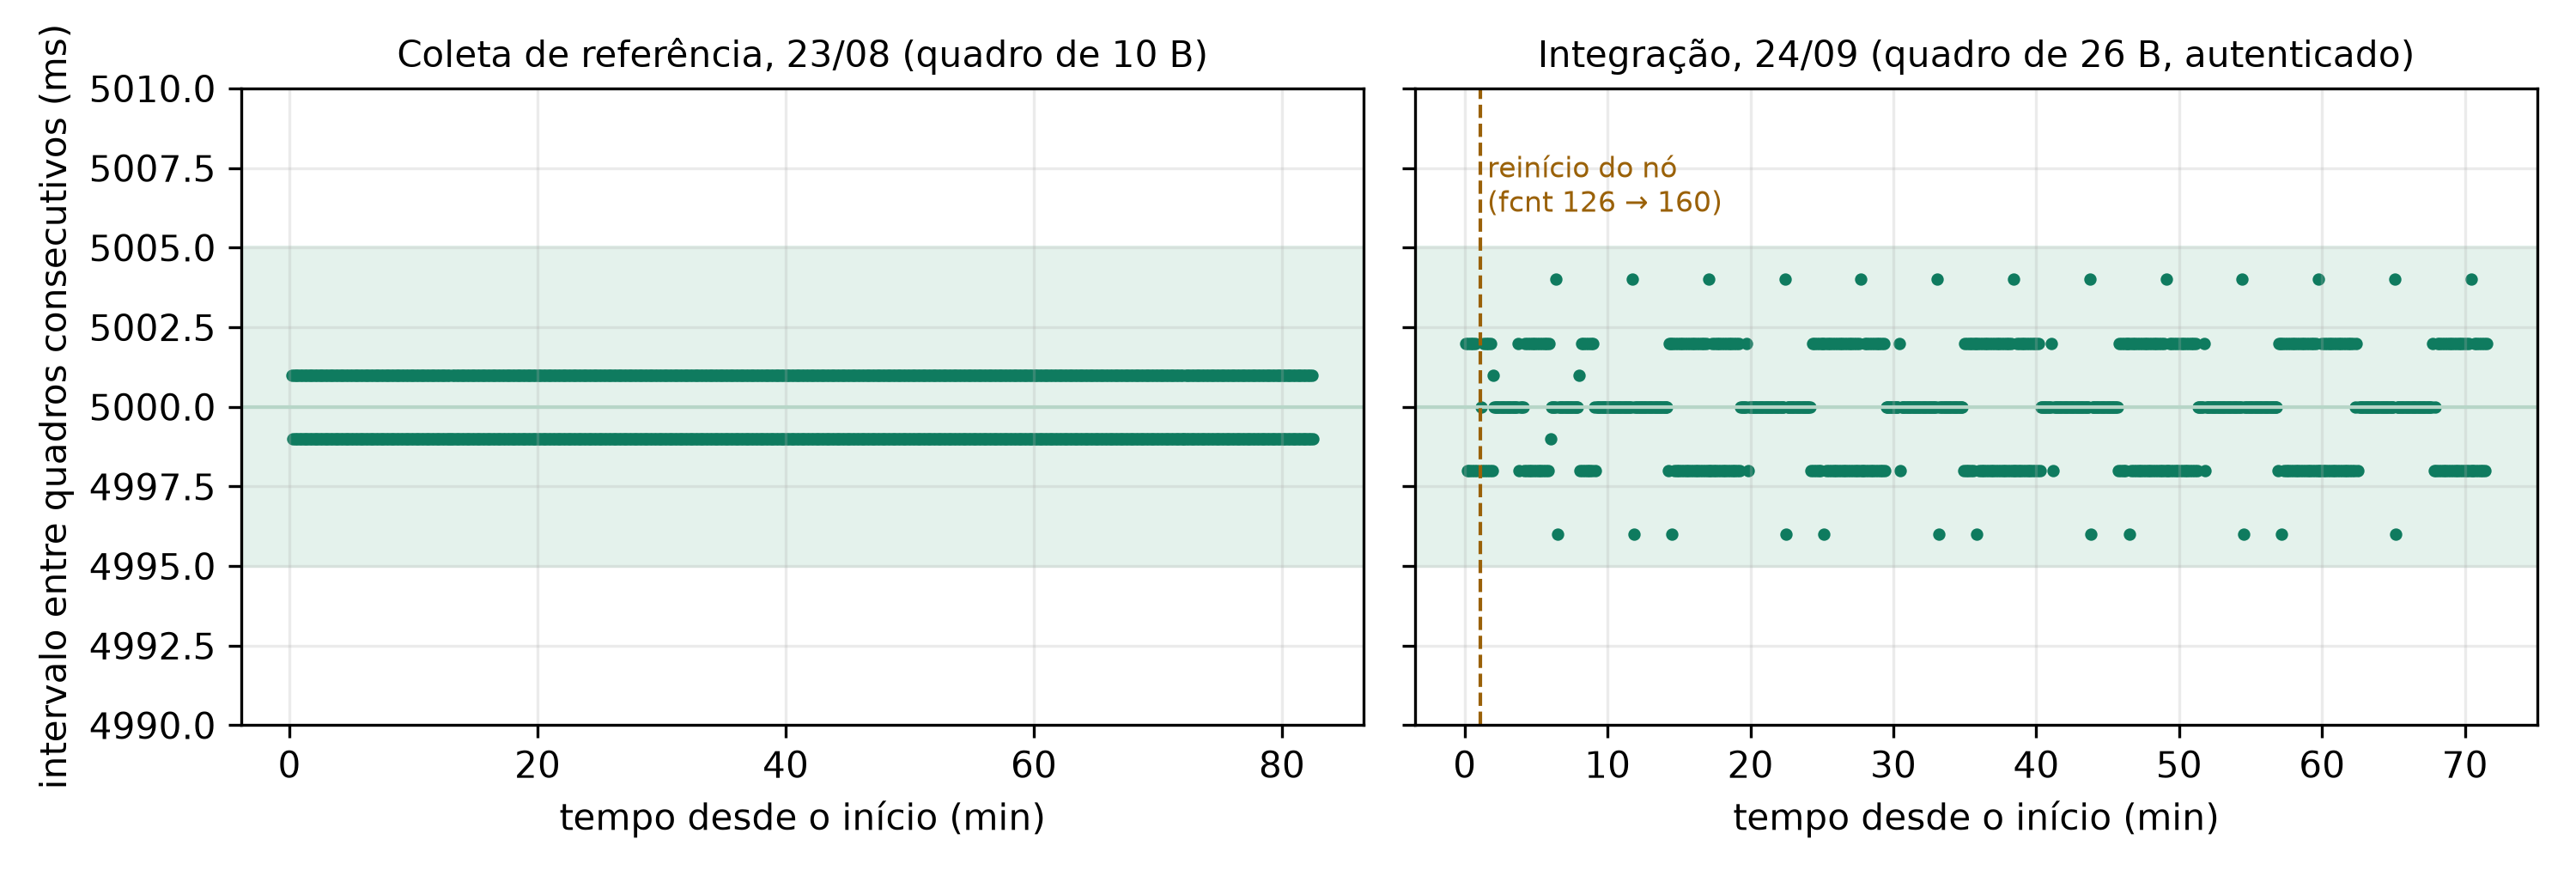
\includegraphics[width=\textwidth]{barea/figuras/cadencia_coletas.png}
  \end{center}
  \legend{Fonte: elaborado pelos autores (2026). A faixa sombreada indica $\pm 5$ ms em torno do período. A linha tracejada marca o reinício do nó.}
\end{figure}

A Figura~\ref{fig:cadencia_coletas} mostra o intervalo entre quadros consecutivos ao longo das duas coletas. Em nenhuma delas houve perda de rádio, e a cadência ficou dentro de $\pm 5$~ms do período em todos os quadros. O desvio padrão maior na segunda coleta (1,56 contra 1,00 ms) é compatível com o processamento adicional nas duas pontas, a cifragem no nó e a atividade de Wi-Fi no 	extit{gateway}, mas atribuí-lo a uma delas exigiria medição dedicada, com carimbo de tempo de microssegundo.

\begin{figure}[htb]
  \caption{\label{fig:rssi_integracao}RSSI por quadro na coleta de 24 de setembro}
  \begin{center}
      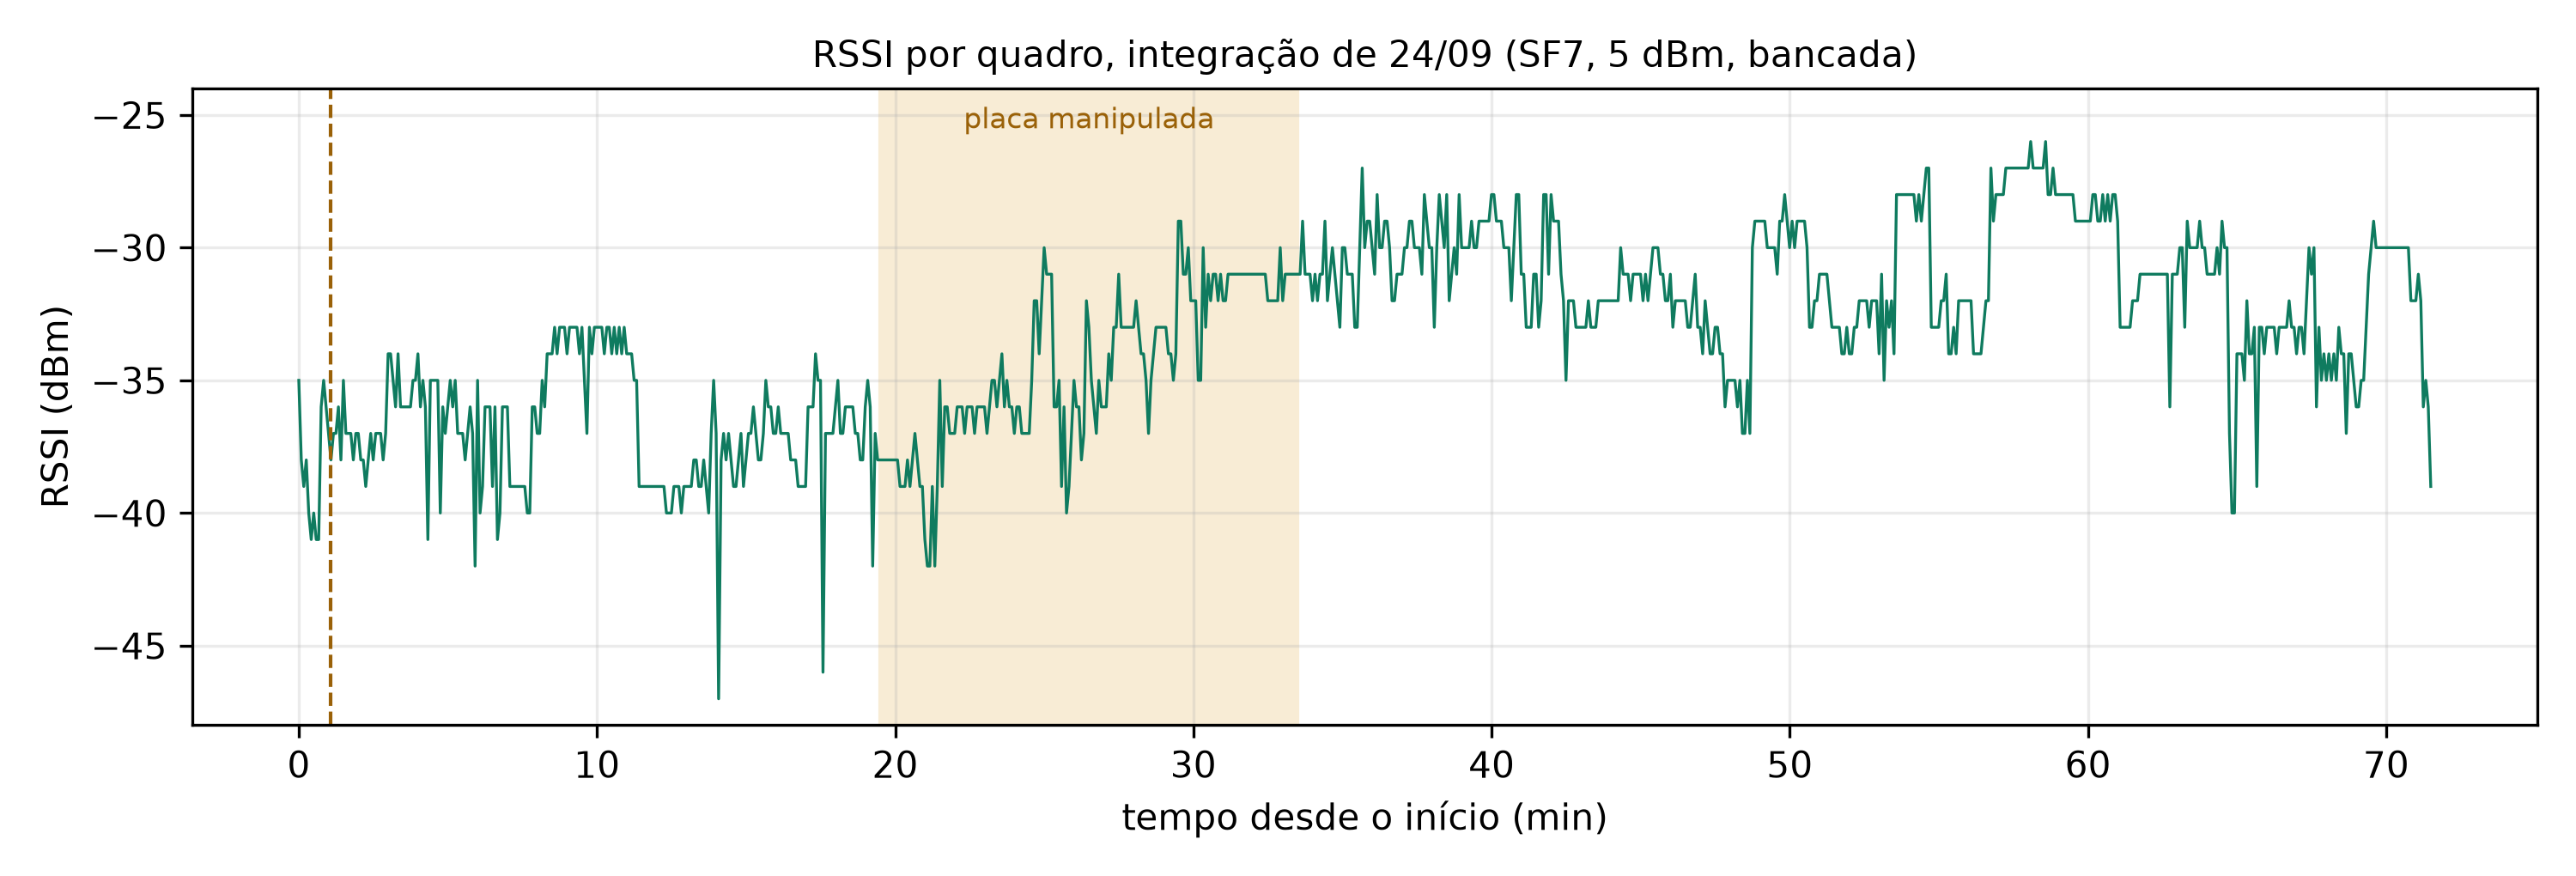
\includegraphics[width=\textwidth]{barea/figuras/rssi_integracao.png}
  \end{center}
  \legend{Fonte: elaborado pelos autores (2026). A área sombreada indica o período em que a placa do nó foi manipulada.}
\end{figure}

\subsection{Discussão}

\textbf{Reinício do nó e perda de rádio.} Na coleta de 24 de setembro, o contador saltou de 126 para 160 com intervalo de 14,7~s entre os dois quadros. Uma contagem simples registraria 33 quadros perdidos, ou 3,7\% de perda. A perda real de 33 quadros teria produzido um intervalo de cerca de 170~s; o intervalo observado e o fato de 160 ser múltiplo de 32 identificam um reinício do nó. A regra que separa os dois casos foi incorporada à API e à ferramenta de análise depois desse achado, e é o motivo de a Tabela~\ref{tab:coletas} distinguir "pulados" de "perdidos". Para a frente de aprendizado de máquina, a distinção importa: um reinício é um evento do dispositivo, uma perda é um evento do enlace, e um detector treinado sem essa separação aprenderia a confundir os dois.

\textbf{Mudança de regime no RSSI.} A Figura~\ref{fig:rssi_integracao} mostra o RSSI em torno de $-37$~dBm nos primeiros vinte minutos e entre $-30$ e $-33$~dBm a partir do trigésimo quarto, com uma transição no intervalo em que a placa do nó foi manipulada. Não é um fenômeno de rede: é a posição da antena. O episódio ilustra o que os modelos precisam distinguir: uma mudança de regime causada por intervenção física produz uma série que um detector de anomalias marcaria, e só o contexto operacional permite rotulá-la corretamente.

\textbf{SNR saturado.} Nas duas coletas o SNR variou menos de 3~dB enquanto o RSSI variou mais de 15~dB, sem correlação entre os dois. Com as placas a poucos metros, o estimador de SNR do transceptor opera saturado, como discutido na Subseção~\ref{subsec:camada_fisica_lora}. Em bancada, o SNR é uma coluna quase constante e não tem valor como variável de entrada; ele só passa a variar de forma útil em testes de alcance.

\textbf{Tempo no ar.} O tempo no ar calculado pela fórmula do fabricante para o quadro de 26 bytes em SF7 é de 61,7~ms, e para o quadro de 10 bytes, 41,2~ms. O tempo medido da função de transmissão, do início da chamada ao fim da transmissão, foi de 69 e 48~ms, respectivamente. A diferença de cerca de 7~ms é constante e corresponde ao processamento fora do rádio: montagem do quadro, cifragem e carga do transceptor. A camada de segurança acrescentou 50\% ao tempo no ar (de 41,2 para 61,7~ms), quase todo devido à tag de autenticação de 16 bytes; derivar o \textit{nonce} em vez de transmiti-lo evitou outros 16 bytes, que elevariam o tempo no ar a 87,3~ms.

\textbf{Limitações.} Uma coleta com perda zero valida a infraestrutura, mas é o caso em que nada está errado: quase toda a variabilidade que um detector precisa aprender está ausente, e as coletas apresentadas servem como referência de comportamento normal, não como conjunto de treinamento. Os dados de aplicação são sintéticos. A janela anti-replay do \textit{gateway} vive em memória volátil: um reinício do \textit{gateway} a zera, e há uma janela de repetição possível até a chegada do primeiro quadro válido, limitação que o LoRaWAN resolve persistindo o contador no \textit{network server}. Todos os nós compartilhariam uma mesma chave, ao contrário do LoRaWAN, em que cada dispositivo tem a sua. A medição de energia do nó e o teste de alcance com fatores de espalhamento maiores não foram executados.


%%%%%%%%%%%%%%%%%%%%%%%%%%%%%%%%%%%%%%%%%%%%%%%%%%%%%%
%%%%%%%%%%%%%%%%%%%%%%%%%%%%%%%%%%%%%%%%%%%%%%%%%%%%%%
